% Research trajectory, not a quantitative comparison of model accuracy.
\documentclass[tikz,border=4pt]{standalone}
\usepackage[T1]{fontenc}
\usepackage{lmodern}
\usetikzlibrary{arrows.meta}
\begin{document}
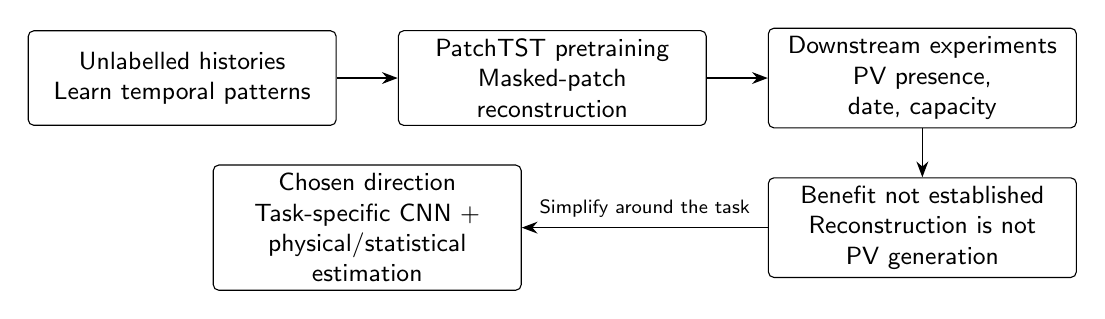
\begin{tikzpicture}[font=\sffamily\small,
 box/.style={draw,rounded corners=2pt,align=center,text width=37mm,minimum height=12mm,inner sep=3pt},
 flow/.style={-{Stealth[length=2mm]},semithick}]
\node[box] (data) at (0,0) {Unlabelled histories\\Learn temporal patterns};
\node[box] (ssl) at (4.7,0) {PatchTST pretraining\\Masked-patch\\reconstruction};
\node[box] (transfer) at (9.4,0) {Downstream experiments\\PV presence, date, capacity};
\node[box] (limits) at (9.4,-1.9) {Benefit not established\\Reconstruction is not\\PV generation};
\node[box] (chosen) at (2.35,-1.9) {Chosen direction\\Task-specific CNN +\\physical/statistical estimation};
\draw[flow] (data) -- (ssl);
\draw[flow] (ssl) -- (transfer);
\draw[flow] (transfer) -- (limits);
\draw[flow] (limits) -- node[above,font=\sffamily\scriptsize] {Simplify around the task} (chosen);
\end{tikzpicture}
\end{document}
